%!TEX root = ../report.tex

\section{Design Pattern}


\subsection{Structural Pattern}

\subsubsection{Adapter Pattern/Wrapper}
Connects incompatible components to for example
\begin{itemize}
  \item Reuse existing components
  \item Convert an interface to another interface (maybe needed by an API call)
\end{itemize}

Structure:\\
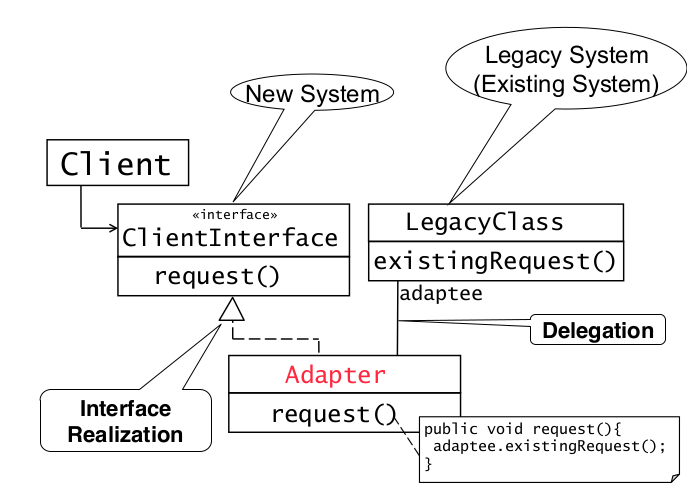
\includegraphics[width=\linewidth]{images/pattern_adapter.png}
\newpage

\subsubsection{Bridge Pattern}
Allows to delay the assignment of an implementation of an interface from compile to run time.\\
Structure:\\
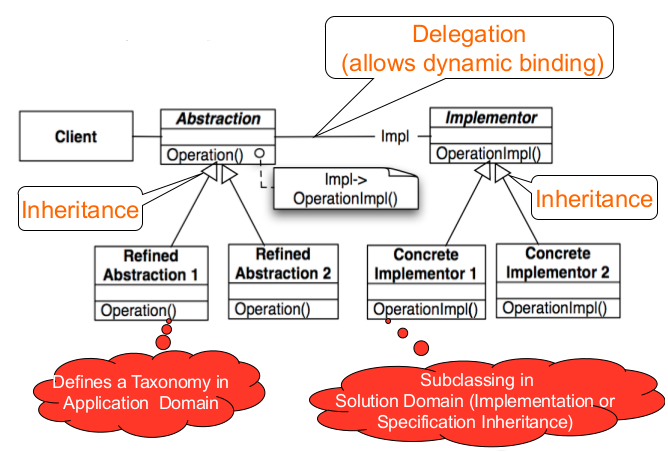
\includegraphics[width=\linewidth]{images/pattern_bridge.png}
The \textbf{degenerated bridge pattern} is the same as the bridge pattern without the taxonomy in the application domain.
\newpage

\subsubsection{Proxy Pattern/Caching}
The proxy pattern allows to defer object creation and object initialization to the time you need the object (Remote Proxy (Caching), Substitute (Virtual Proxy), Protection Proxy (Access control/Firewall)).\\
Structure:\\
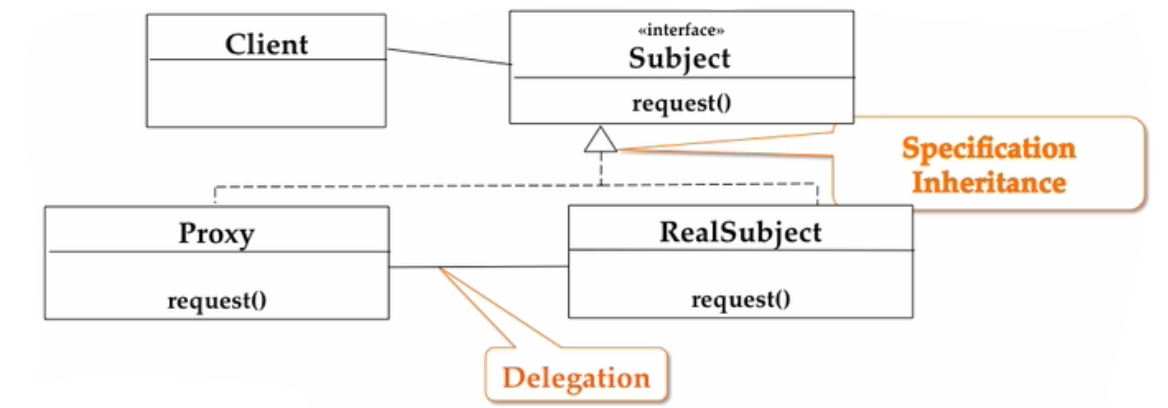
\includegraphics[width=\linewidth]{images/pattern_proxy.png}
The client never calls request() in RealSubject, instead it always calls the method in Proxy which might delegate it to the RealSubject.
\newpage

\subsubsection{Composite Pattern}
The composite pattern models tree structures that represent part-whole hierarchies with arbitrary depth and width.
It lets the client treat individual objects and groups uniformly. \\
Structure:\\
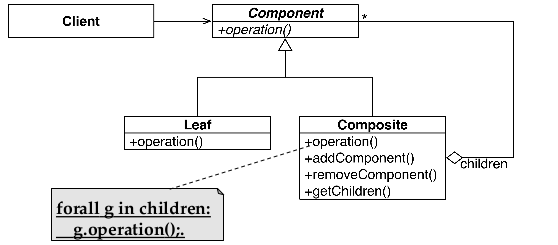
\includegraphics[width=\linewidth]{images/pattern_composite.png}
\newpage


\subsection{Behavioral Pattern}

\subsubsection{Strategy Pattern}
Suited for situations where different algorithms are available for a problem (e.g. sorting).\\
Structure:\\
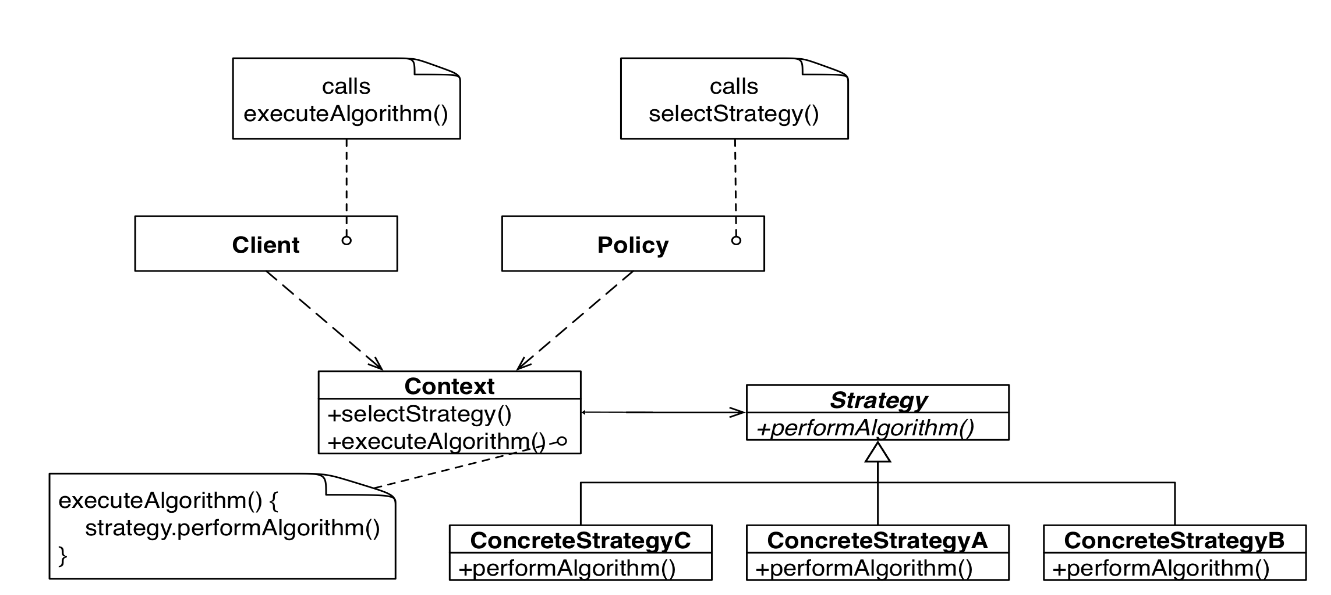
\includegraphics[width=\linewidth]{images/pattern_strategy.png}
A strategy is chosen on \textbf{runtime} by the Policy class before the client calls executeAlgorithm.
\newpage

\subsubsection{State Pattern}
Dependent on the current state of a system, an action should do different things (e.g. TCP open, close).
The state pattern avoids many if else statements and is flexible to add more cases/states.\\
Structure:\\
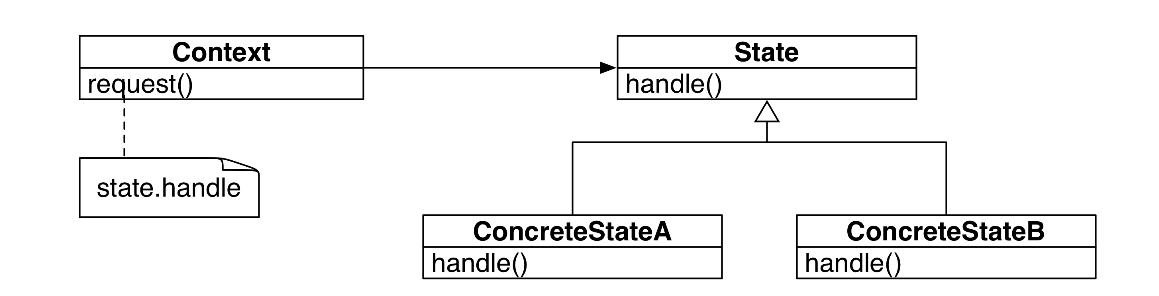
\includegraphics[width=\linewidth]{images/pattern_state.png}
Problem: Where are state transactions handled? (in the exercise of the lecture in the states)
\newpage

\subsubsection{Observer Pattern}
The observer pattern handles changes in a publisher class and notifies all subscribers about that change (e.g. the user interface) to maintain consistency.
There are three variants for maintaining consistency:
\begin{itemize}
  \item \textbf{Push Notification:} Every time a state changes, all subscribers are notified
  \item \textbf{Push-Update Notification:} The publisher also sends the state that has changed
  \item \textbf{Pull Notification:} A subscriber inquires about the state of the publisher
\end{itemize}
Structure:\\
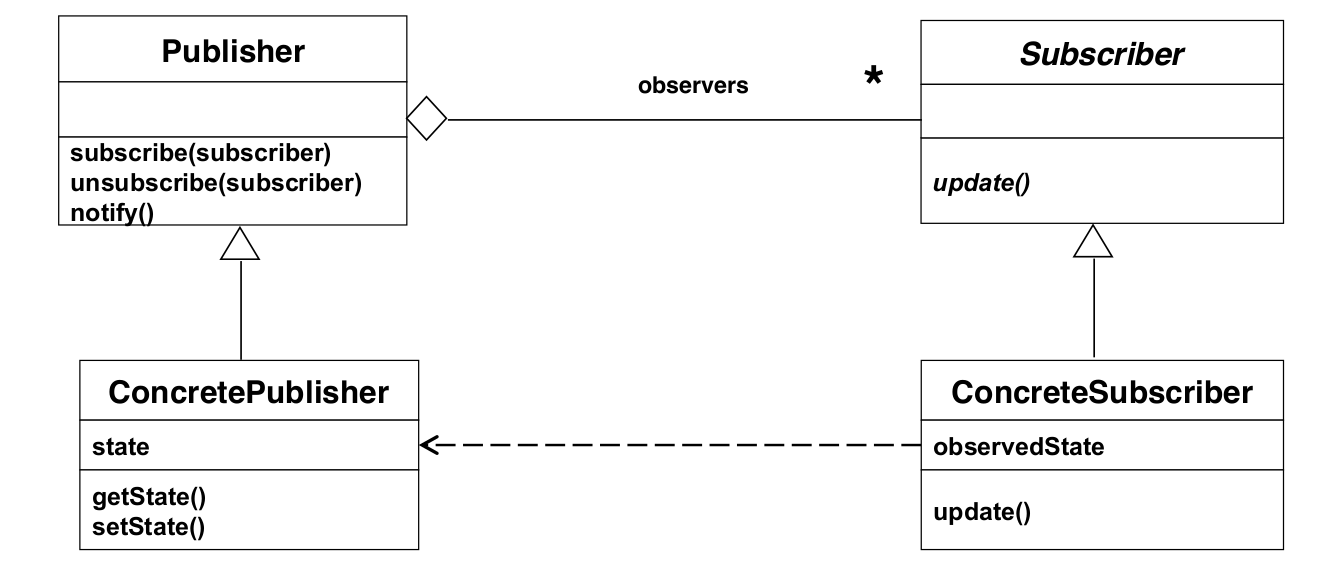
\includegraphics[width=\linewidth]{images/pattern_observer.png}
\newpage

\subsubsection{Model View Controller Pattern}
The model-view-controller architectural style decouples data access and data representation.
The view handles the data representation, the model the data access and the controller handles the communication between the other two.\\
Structure:\\
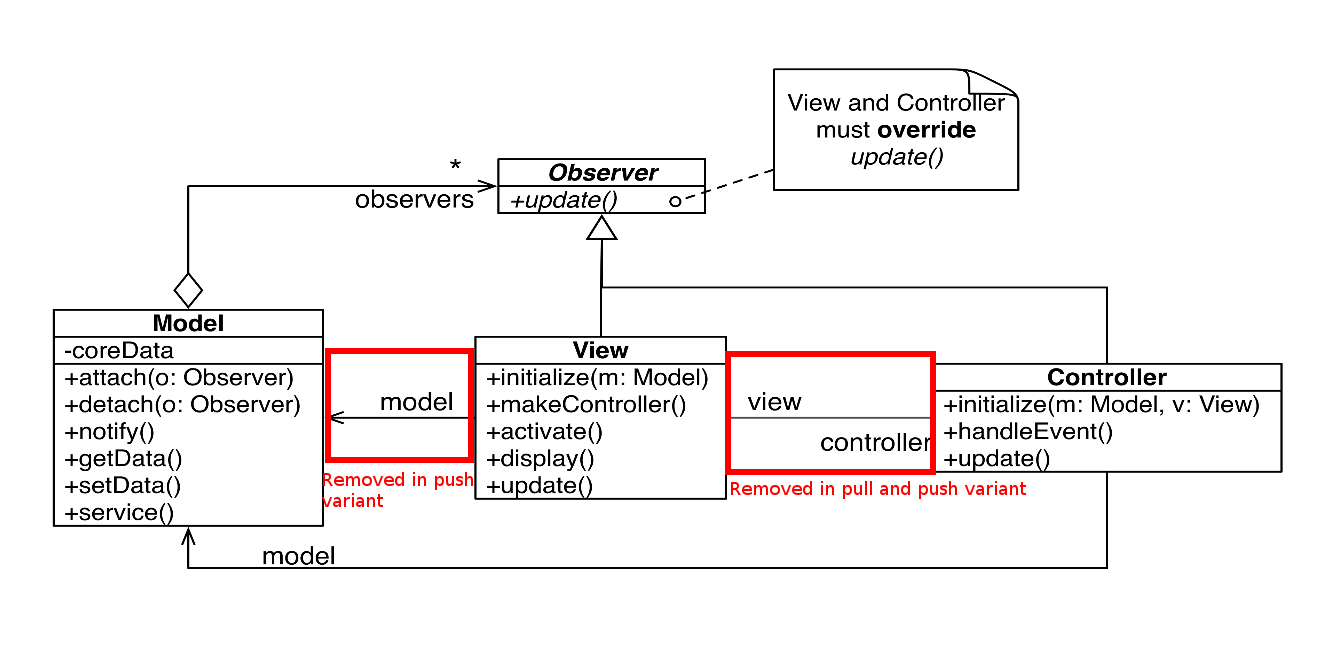
\includegraphics[width=\linewidth]{images/pattern_mvc.png}
In the \textbf{pull variant} the connection between the controller and the view is removed.
In this variant the view asks the model for the data explicitly.\\
In the \textbf{push notification variant} both the connection between the view and the model and controller respectively are removed.
When a change in the model occurs, the view and the controller are updated via the observer pattern.

\subsubsection{Command Pattern}
The command pattern is used for designing user interfaces with multiple commands without using multiple if statements (if(command == x) {...} else if(command == y) ...).
It can be used to make menus reusable across applications.\\
Structure:\\
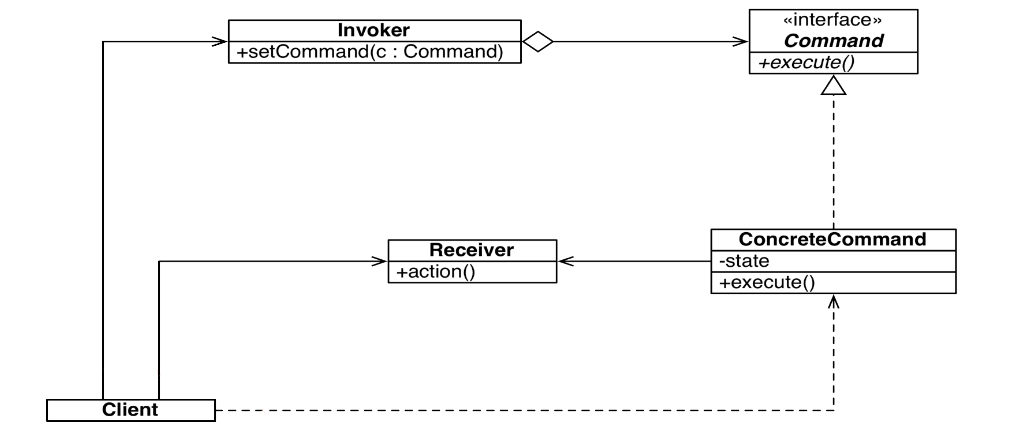
\includegraphics[width=\linewidth]{design_pattern/command.png}
Commands as classes allow command histories and thus undo and redo.\\
Common Applications:
\begin{itemize}
  \item \textbf{Command Manager} Central repository for all commands
  \item \textbf{Redo/Undo Manager}
  \item \textbf{Queue} Holds commands until others objects are ready to do something with them
  \item \textbf{Dispatcher} (e.g. keyboard event loop)
\end{itemize}
